% A halo model for intrinsic alignments with nonlinear halo bias in the
% 2-halo term, and a prototype test against FLAMINGO.
% Build with .claude/skills/summary-notes/assets/build_note.sh analysis/halo_nlbias
\documentclass[11pt]{article}

\usepackage[margin=1in]{geometry}
\usepackage{amsmath}
\usepackage{amssymb}
\usepackage{graphicx}
\usepackage{booktabs}
\usepackage{xcolor}
\usepackage{enumitem}
\usepackage[font=small,labelfont=bf,labelsep=period]{caption}
\usepackage[hidelinks]{hyperref}

% Symbols, one macro per object.
\newcommand{\hMpc}{\,h\,{\rm Mpc}^{-1}}
\newcommand{\Msun}{\,h^{-1}M_\odot}
\newcommand{\Plin}{P_{\rm lin}}
\newcommand{\PNL}{P_{\rm NL}}
\newcommand{\bTA}{b_{\rm TA}}
\newcommand{\bNL}{\beta_{\rm NL}}
\newcommand{\Cb}{\bar C_1}
\newcommand{\Cbb}{\bar C_2}
\newcommand{\kmax}{k_{\max}}
\newcommand{\dd}{\mathrm{d}}
\newcommand{\nbar}{\bar n}
\newcommand{\Ib}[1]{I^{\beta}_{#1}}

% =====================================================================
% Numbers
% =====================================================================
% Every number the text quotes is defined here, with the file (and key)
% it comes from. Part 1: results, refreshed when the analysis is rerun;
% set \numbersfinalfalse to print them in red while they are stale.
% Part 2: inputs, which a rerun does not change.
%
% Statements of the text that rest on Part 1 (re-check after a refresh):
%   - beta_NL alone does not replace alpha beyond k_max ~ 0.5 (Summary,
%     section "Fits without alpha").
%   - the held low-mass beta_NL matches FLAMINGO's P_gm to < 8 percent and
%     the lower bracket does not (section "A check on FLAMINGO's clustering").
%   - the beta_NL share of the alpha correction rises with z and falls above
%     k ~ 0.7 (section "beta_NL and the 2-halo gap").
\newif\ifnumbersfinal
\numbersfinaltrue
\newcommand{\refresh}[1]{\ifnumbersfinal#1\else\textcolor{red}{#1}\fi}
% Part 1: results.
% summed chi2/nu over the nine core snapshots at k_max = 0.52, 0.70, 0.94
% (nlbias_numbers.json, gof)
\newcommand{\GofAlpha}{\refresh{0.97, 1.08 and 1.33}}
\newcommand{\GofNlb}{\refresh{1.49, 4.08 and 15.9}}
\newcommand{\GofNlbTT}{\refresh{3.46, 17.6 and 88.8}}
\newcommand{\GofNlbSat}{\refresh{1.54, 3.70 and 10.7}}
\newcommand{\GofLin}{\refresh{2.10, 4.79 and 12.7}}
\newcommand{\GofNlbNLA}{\refresh{9.8, 40 and 157}}
\newcommand{\GofAlphaNLA}{\refresh{1.77, 2.58 and 3.94}}
\newcommand{\GofNlbLo}{\refresh{16, 60 and 199}}
% the beta_NL share of the alpha correction, I^beta_cm / [alpha (P_NL/P_lin - I_1)],
% alpha of alpha_tatt at k_max = 0.70 (nlbias_numbers.json, gap)
\newcommand{\ShareLowZ}{\refresh{0.55 to 0.69}}
\newcommand{\ShareMidZ}{\refresh{0.75 to 0.96}}
\newcommand{\ShareHighZ}{\refresh{1.1 to 1.3}}
\newcommand{\ShareHighK}{\refresh{0.31 to 0.77}}
% the alpha implied by beta_NL at k = 0.39 (share x alpha), z = 0.2 and z = 1
\newcommand{\AlphaBetaLowZ}{\refresh{0.26}}
\newcommand{\AlphaBetaZone}{\refresh{0.72}}
% I^beta_cm at k = 0.1 (nlbias_numbers.json, gap, Ib_cm_k0.1)
\newcommand{\IbLowK}{\refresh{$-0.02$ to $-0.04$}}
% FLAMINGO clustering checks, model/FLAMINGO over k = 0.29 to 0.94
% (nlbias_numbers.json, checks)
\newcommand{\PgmNlb}{\refresh{0.98 to 1.07}}
\newcommand{\PgmPlain}{\refresh{0.62 to 0.88}}
\newcommand{\PgmLo}{\refresh{0.66 to 0.90}}
\newcommand{\PggNlbZone}{\refresh{1.04 to 1.16}}
\newcommand{\PggPlainZone}{\refresh{0.86 to 0.92}}
\newcommand{\PmmNlbZone}{\refresh{0.96 to 1.03}}
\newcommand{\PmmPlainZone}{\refresh{0.70 to 0.90}}
\newcommand{\PmmNlbZlow}{\refresh{0.89 to 0.97}}
% fitted parameters of nlb_tatt (nlbias_numbers.json, params)
\newcommand{\AoneRatioNlb}{\refresh{1.00 to 1.06}}
\newcommand{\AoneRatioNlbHigh}{\refresh{0.88 to 0.97}}
\newcommand{\bTANlbLow}{\refresh{0 to 0.38}}
\newcommand{\bTANlbHigh}{\refresh{0.48 to 0.74}}
% b_TA of alpha_tatt at k_max = 0.94
\newcommand{\bTAAlpha}{\refresh{0.13 to 0.87}}
% satellite amplitudes of nlb_tatt_sat at k_max = 0.39 to 0.94 where not 0
\newcommand{\AoneHSat}{\refresh{0.09 to 2.4}}
% number of best fits (of 117 per variant) with a sign change of the GI or II
% 2-halo term at k >= 3.04, and the lowest such k (nlbias_numbers.json, signs)
\newcommand{\NSignGI}{\refresh{45}}
\newcommand{\NSignII}{\refresh{24}}
% Part 2: inputs.
\newcommand{\Mlow}{10^{12.5}}

\begin{document}

\begin{center}
  {\LARGE Nonlinear halo bias in the halo model\\[0.2em] for intrinsic alignments\par}
  \vspace{0.6em}
  {\large Can $\bNL$ replace the free nonlinear share $\alpha$ of the HMc refit?\par}
  \vspace{0.6em}
  {\large November 2026\par}
  \ifnumbersfinal\else
    \vspace{0.6em}
    {\color{red}Numbers in red are being refreshed.\par}
  \fi
\end{center}
\vspace{1em}

\section{Summary}
\label{sec:summary}

\paragraph{The question.}
The halo model with a central 1-halo term (HMc) fits the FLAMINGO intrinsic
alignment (IA) spectra to $k \sim 1\hMpc$ only when a free share $\alpha$ of
the nonlinear matter power is added to its 2-halo term. Can the nonlinear
halo bias $\bNL(k, M_1, M_2)$ of Mead \& Verde (arXiv:2011.08858), a
physical correction to the 2-halo term, replace $\alpha$?

\paragraph{The answer.}
Only up to $k \approx 0.5$ to $0.7\hMpc$. With $\bNL$ from Dark Emulator, the
2-halo GI term carries \ShareLowZ{} of the $\alpha$ correction at
$z = 0.2$ to 0.3, \ShareMidZ{} at $z = 0.4$ to 0.5 and \ShareHighZ{} at
$z = 0.6$ to 1 for $k = 0.3$ to $0.5\hMpc$, but it turns over above
$k \approx 0.7$ (halo exclusion) while FLAMINGO keeps rising like $\PNL$. Without $\alpha$, with $a_c \le 1$, the
summed $\chi^2/\nu$ over the nine core snapshots at $\kmax = 0.52$, 0.70 and
0.94 is \GofNlb{}, against \GofAlpha{} for the $\alpha$ refit and \GofLin{}
for HMc (Fig.~\ref{fig:gof}).

\paragraph{What failed.}
\begin{itemize}[itemsep=1pt,topsep=2pt]
  \item \emph{The fit beyond $\kmax \approx 0.5$.} The missing power at
    $k \gtrsim 0.7$ has the shape of $\PNL$, i.e.\ of 1-halo power, which no
    2-halo correction supplies. The physical 1-halo terms do not supply it
    either: $a_c$ sits at its bound of 1, and the F21 satellites give
    \GofNlbSat{} with an amplitude $a_{1h}$ that is unconstrained and
    unphysical (Section~\ref{sec:fits}, Fits without $\alpha$).
  \item \emph{Drift.} With $\bNL$, $\bTA$ rises from \bTANlbLow{} at
    $\kmax \le 0.52$ to \bTANlbHigh{} at 0.94, and $A_1$ falls to
    \AoneRatioNlbHigh{} of its low-$k$ NLA value: both compensate for the
    missing high-$k$ power. Below $\kmax = 0.70$, $A_1$ is \AoneRatioNlb{}
    times the NLA value, about 4 at $z = 1$ (passes).
  \item \emph{Without $\bTA$} (the choice motivated in
    Section~\ref{sec:tatt}) the fit is much worse, \GofNlbTT{}, and $A_2$
    flips sign. The data keep wanting the density-weighting term.
  \item \emph{Mass coverage.} Dark Emulator is stable only above
    $n(>M) = 10^{-2.9}\,h^3{\rm Mpc}^{-3}$, i.e.\ $M \gtrsim 10^{12.6}\Msun$,
    while most FLAMINGO centrals sit at $10^{11.5}$ to $10^{12.5}$. $\bNL$ is
    held at its lowest-mass value below that (Mead \& Verde's choice); with
    $\bNL = 0$ there instead, the correction vanishes. The $z = 1.5$ and 2
    tables are extrapolated from $z = 1.48$.
  \item \emph{Low $k$.} $\Ib{cm} = \IbLowK$ at $k = 0.1\hMpc$, a dip that
    $\PNL$ does not have (unequal-mass pairs in the emulator).
\end{itemize}

\paragraph{What worked.}
The model reduces to NLA (TATT with $\bTA = 0$) at low $k$ by construction.
On FLAMINGO's own galaxy-matter spectrum at $z = 1.5$ and 2 the held $\bNL$
gives \PgmNlb{} of the measured $P_{gm}$ at $k = 0.3$ to 0.9, against
\PgmPlain{} without $\bNL$ and \PgmLo{} with $\bNL = 0$ below the emulator's
masses (Fig.~\ref{fig:checks}). The $\alpha$ that $\bNL$ implies at
$k = 0.39$ rises from \AlphaBetaLowZ{} at $z = 0.2$ to \AlphaBetaZone{} at
$z = 1$: the rise of the fitted $\alpha$ with redshift is the rise of
nonlinear halo bias.

\paragraph{Limits.} FLAMINGO's errors are underestimated by 3 to 9 times at
high $k$, so the $\chi^2$ values compare models with each other and are not
goodness of fit at $k \gtrsim 1$. The FLAMINGO galaxy spectrum $P_{gg}$ at
$z = 1$ is overpredicted by the held $\bNL$ (\PggNlbZone{}), which mixes the
$\bNL$ extrapolation with the HOD's 1-halo term. The cross of halo shapes with
halo density is assumed to carry the same $\bNL$ as halo density
(Section~\ref{sec:model}).

\section{Setup}
\label{sec:setup}

\paragraph{Data.} FLAMINGO L1\_m8 IA spectra $P_{hE}$, $P_{EE}$, $P_{BB}$ at
$\mu = 0$ in the cosmolike convention, nine core snapshots $z = 0.2$ to 2
(\texttt{analysis/roman\_dchi2/v2/fits.npz}), with FLAMINGO's error bars and
$0.05 \le k \le \kmax$. $P_{hE} = b(k)P_{\delta E}$ with the measured
$b(k) = (P_{hh}/\PNL)^{1/2}$, the convention of the Roman truth. Cosmology
FLAMINGO D3A ($h = 0.681$, $\Omega_m = 0.306$, $\Omega_b = 0.0486$,
$n_s = 0.967$, $A_s = 2.099\times10^{-9}$, $m_\nu = 0.06$\,eV).

\paragraph{Halo model.} As HMc (\texttt{analysis/roman\_dchi2/v6/halo\_ia.py}):
CAMB linear CDM plus baryon power, Tinker et al.\ (2010) mass function and
bias at $\Delta = 200\bar\rho_m$, Bhattacharya et al.\ (2013) concentrations,
NFW profiles $u(k|M)$, and an HOD per snapshot,
$N_c = \tfrac12[1 + {\rm erf}((\lg M - \lg M_{\min})/0.25)]$,
$N_s = N_c(M - M_{\min})/M_1$, with $(M_{\min}, M_1)$ set by the sample's
$\nbar_g$ and large-scale $b_g$.

\paragraph{Fits.} Everything but the spectra under the $A_1$ terms is the
$\alpha$ refit (\texttt{hmc\_alpha\_fit.py}, variant
\texttt{alpha\_cap\_nosat}): $N_s$ fixed, a free white term $W$, the central
1-halo amplitude $a_c \in [0, 1]$, no satellites unless stated, the window
$f_{2h} = e^{-(k/6)^2}$. The $\alpha$ refit is reproduced to 0.01 in summed
$\chi^2/\nu$. The statistic is $\sum_z\chi^2_{\min}/\sum_z\nu$ over the nine
snapshots.

\section{The model}
\label{sec:model}

\subsection{2-halo terms with nonlinear halo bias}

Following Mead \& Verde, the 2-halo spectrum of two fields $X$ and $Y$ is
\begin{equation}
P^{2h}_{XY}(k) = \Plin(k)\!\int\!\dd\ln M_1\,\dd\ln M_2\; n_1 n_2\, b_1 b_2\,
W_X(M_1, k)\,W_Y(M_2, k)\,\big[1 + \bNL(k, M_1, M_2)\big],
\label{eq:2h}
\end{equation}
with $n = \dd n/\dd\ln M$, $b(M)$ the linear halo bias, $W$ the kernel of
each field per halo, and
\begin{equation}
\bNL(k, M_1, M_2) = \frac{P_{hh}(k | M_1, M_2)}{b(M_1)\,b(M_2)\,\Plin(k)} - 1
\label{eq:beta}
\end{equation}
the departure of the halo-halo spectrum from linear bias, halo exclusion
included. The kernels are
\begin{equation}
W_m = \frac{M}{\bar\rho}\,u(k|M),\qquad
W_g = \frac{N_c + N_s\,u(k|M)}{\nbar_g},\qquad
W_c = \frac{N_c\,w(M)}{\nbar_c\,b(M)},\quad
\int\!\dd\ln M\,n\,N_c\,w = \nbar_c ,
\end{equation}
for matter, galaxy positions and central shapes. Eq.~\eqref{eq:2h} splits
into the linear part and a $\bNL$ part,
$P^{2h}_{XY} = \Plin[I_X I_Y + \Ib{XY}]$, with $I_X = \int n\,b\,W_X$ and
$\Ib{XY}$ the double integral with $\bNL$.

\paragraph{How the central alignment enters.} A central in a halo of mass $M$
has the intrinsic shear $\gamma_{ij} = -A_1\Cb\,w(M)\,s_{ij}$, with $s_{ij}$
the large-scale tidal field felt by the halo. Its cross spectrum with halos of
mass $M_2$ is $b_K(M)\,b(M_2)\Plin[1 + \beta^{K h}]$, with the shape bias
$b_K \propto w$. The model assumes $\beta^{Kh} = \bNL$: halo shapes inherit
the nonlinear clustering of the halo positions. The fiducial weight is
$w = b(M)/\bar b_c$ (shape bias proportional to density bias, as FLAMINGO's
$A_1/b_g$ is constant across snapshots); $w = 1$ is the variant~T. The central
shape kernel per unit $-A_1\Cb$ is normalised so that $I_c = 1$, so $A_1$ is
the large-scale NLA amplitude per galaxy (the central fraction is absorbed in
it, as in HMc).

\paragraph{The spectra.}
\begin{align}
P^{2h}_{\delta E} &= -A_1\Cb\,\Plin\big[I_1(k) + \Ib{cm}(k)\big]
  - A_1\Cb\bTA K_{\delta E} + 5A_2\Cbb K_{\rm mix},\label{eq:gi}\\
P^{2h}_{EE} &= A_1^2\Cb^2\,\Plin\big[1 + \Ib{cc}(k)\big]
  + A_1^2\Cb^2\big(\bTA^2K_{\rm ta} + 2\bTA K_{\delta E}\big)\nonumber\\
  &\quad - 10A_1A_2\Cb\Cbb\big(K_{\rm mix} + \bTA K_{\rm mixEE}\big) + 25A_2^2\Cbb^2K_{\rm tt},\label{eq:ii}\\
P^{2h}_{BB} &= A_1^2\Cb^2\bTA^2K_{\rm taBB} - 10A_1A_2\Cb\Cbb\bTA K_{\rm mixBB}
  + 25A_2^2\Cbb^2K_{\rm ttB},\label{eq:bb}\\
P^{2h}_{hE} &= -A_1\Cb\,\Plin\big[b_g(k) + \Ib{gc}(k)\big] + \dots,
  \qquad b_g(k) = I_g(k),\label{eq:he}
\end{align}
with $\Cb = 0.01389\,\Omega_m/D(z)$, $\Cbb = 0.01389\,\Omega_m/D^2(z)$, the
FAST-PT one-loop kernels $K_X(k)$ and $I_1 = I_m$ as in HMc. Explicitly,
\begin{align}
\Ib{cm}(k) &= \int\!\dd\ln M_1\,\dd\ln M_2\; n_1 n_2\,\frac{N_c(M_1)\,w(M_1)}{\nbar_c}\,
b_2\,\frac{M_2}{\bar\rho}\,u(k|M_2)\,\bNL(k, M_1, M_2),\\
\Ib{cc}(k) &= \int\!\dd\ln M_1\,\dd\ln M_2\; n_1 n_2\,\frac{N_c(M_1)\,w(M_1)}{\nbar_c}\,
\frac{N_c(M_2)\,w(M_2)}{\nbar_c}\,\bNL(k, M_1, M_2).
\end{align}
The GI term is the central-matter 2-halo spectrum weighted by $N_c w$, the II
term the central-central one. $\bNL$ is a correction to a scalar (the tidal
field's source), so it creates no $B$ mode: $P_{BB}$ is unchanged. The
galaxy-shape spectrum Eq.~\eqref{eq:he} is the form for a fit to $P_{hE}$
without the measured $b(k)$; the fits here use $P_{hE} = b(k)P_{\delta E}$ so
that they compare directly with the $\alpha$ refit.

\paragraph{Where $\bNL$ acts.} HMc has $I_1 \simeq 1$ below $k = 1$, so its
GI term is $\Plin$, which at $z = 1$ is 29 to 56\% below $\PNL$ at
$k = 0.39$ to 0.70. $\Ib{cm}$ is 0 at $k \lesssim 0.05$, $\approx 0.15$ to 0.2
at $k = 0.3$, $\approx 0.3$ to 0.5 at $k = 0.5$ and peaks near $k \approx 1$,
where exclusion makes $1 + \bNL$ fall (Fig.~\ref{fig:kernel}). It grows with
redshift at fixed $k$, because the same halos are rarer and more biased.

\subsection{The tidal-torquing and density-weighting terms}
\label{sec:tatt}

$A_2$ (tidal torquing) is quadratic in the tidal field, already a one-loop
term; it keeps its kernels and is not multiplied by $1 + \bNL$. The density
weighting $\bTA$ multiplies the shape field by $1 + \delta$ at the galaxy's
position. In the halo model the shapes sit at halo positions, so their
weighting is the clustering of the host halos, which Eq.~\eqref{eq:2h}
carries through $b(M)$ and $\bNL$; a free $\bTA$ on top counts it twice at one
loop. $\bTA$ was also the parameter that absorbed $\alpha$ (correlation
$-0.85$), and density-weighted terms fail one-loop perturbation theory on
small scales (Harnois-D\'eraps et al.\ 2025, arXiv:2509.25166). The fiducial
of the layout therefore sets $\bTA = 0$; the fits test both.

\subsection{1-halo terms, exclusion and the large-scale limit}

The 1-halo terms are those of HMc, unchanged: the central aligned with its
triaxial halo, $P^{1h,c}_{\delta E} = -a_cP_c(k)$ with $a_c \le 1$
($a_c \approx 0.5$ for a central that copies its halo's shape), no central II
1-halo term, and the radial satellites of Fortuna et al.\ (2021,
arXiv:2003.02700), $P^{1h,s}_{\delta E} = -a_{1h}f_{1h}S_{\delta I}$,
$P^{1h,s}_{EE} = a_{1h}^2f_{1h}S_{II}$. Nothing in $\bNL$ changes them.

Halo exclusion is part of $P_{hh}$ and hence of $\bNL$, so the 2-halo window
$f_{2h}$ is no longer needed for it; it is kept ($f_{2h} \ge 0.97$ for
$k \le 1$) only so that the fits match the $\alpha$ refit.

At low $k$, $u \to 1$, $I_1 \to 1$, $b_g(k) \to b_g$ and $\bNL \to 0$, so
$P_{\delta E} \to -A_1\Cb\Plin + 5A_2\Cbb K_{\rm mix}$ and
$P_{EE} \to A_1^2\Cb^2\Plin + \dots$: NLA for the $A_1$ part, TATT with
$\bTA = 0$ in full. With the emulator, $|\bNL| < 0.02$ below
$k = 0.03\hMpc$ for every mass pair.

\section{Where \texorpdfstring{$\bNL$}{beta\_NL} comes from}
\label{sec:source}

Three sources were considered. Their coverage, against the range of the FLAMINGO sample
(D3A, $z = 0.2$ to 2, centrals from $10^{11.5}\Msun$, $k$ up to 1):

\begin{center}\small
\begin{tabular}{p{2.6cm}p{2.5cm}p{1.9cm}p{3.1cm}p{1.9cm}}
\toprule
source & cosmology & redshift & masses [$\Msun$] & $k$ [$h\,$Mpc$^{-1}$] \\
\midrule
Dark Emulator (\texttt{dark\_emulator}) & wCDM box, D3A inside; $m_\nu = 0.06$\,eV & 0 to 1.48 & $10^{12.6}$ to $10^{14.4}$ (stable part, $z \le 1$) & to $\sim 2$ ($\xi_{hh}$ at $r \ge 0.2$) \\
fitting functions (Tinker et al.\ 2005 $\zeta(r)$; Jose et al.\ 2016) & calibrated at one or few & mainly $z \lesssim 1$ & mass independent, or $b(M)$ only & real space, no exclusion term separately \\
measured in FLAMINGO ($P_{hh}$, $P_{hm}$ per mass bin) & exact & every snapshot & to $\sim 10^{11}$ & to $\sim 3$ \\
\bottomrule
\end{tabular}
\end{center}

\paragraph{Dark Emulator} (Nishimichi et al.\ 2019, arXiv:1811.09504; used by
Mead \& Verde) installs from pip and returns a halo-halo spectrum in 0.05\,s.
Its mass range is set by number density: the direct emulation covers
$n(>M) = 10^{-2.5}$ to $10^{-5.75}\,h^3{\rm Mpc}^{-3}$. Bins that start above
$10^{-2.9}$ are unstable at $z \ge 1$ ($\bNL$ of the lowest bin at $k = 0.1$
moves between $-0.01$ and $-0.13$ with the bin edges), so the usable range is
$M \gtrsim 10^{12.6}\Msun$ at $z = 1$. It stops at $z = 1.48$, and it is
dark-matter only.

\paragraph{Fitting functions} are fast and cover any redshift, but the
standard ones are mass independent (Tinker et al.\ 2005) or give the
halo-matter bias of one mass (Jose et al.\ 2016), in real space, calibrated on
a few cosmologies. None gives $\bNL(k, M_1, M_2)$ with exclusion, which is
what turns the 2-halo term over at $k \sim 1$. One-loop perturbation theory
with coevolution biases covers every mass and redshift but only to
$k \sim 0.2$ to 0.3 at low $z$, below the regime of interest.

\paragraph{Measuring in FLAMINGO} is exact in cosmology, covers every
snapshot and the centrals' masses, and includes baryons. The infrastructure
partly exists: the dark-matter particles were streamed onto the galaxy grids
at $z = 1.5$, 2 and 3 for $P_{gm}$ (\texttt{matter\_cross.py}).

\paragraph{Choice.} Dark Emulator for the prototype; FLAMINGO's own
$P_{hh}(k|M_1, M_2)$ and $P_{hm}(k|M)$ for a production model (see the
Recommendation).

\paragraph{Implementation.} $\bNL$ is computed on nine mass bins between
consecutive thresholds $n(>M) = 10^{-2.9}$ to $10^{-5.6}$, the spectrum of two
bins being the density-weighted combination of four threshold spectra; finite
bins avoid the $\pm1\%$ mass differences of \texttt{get\_phh\_mass}, which are
noisy near the lowest mass. Each pair is normalised by its own amplitude at
$0.01 \le k \le 0.03$ (with the product of the auto-spectrum biases instead,
unequal-mass pairs keep an offset of up to 6\%). On the halo-model mass grid
$\bNL$ is interpolated in $\lg M$ and held at the nearest bin outside the
emulator's range. For $z = 1.5$ and 2 the $z = 1.48$ table is assigned to the
masses of the same peak height.

\section{\texorpdfstring{$\bNL$}{beta\_NL} and the 2-halo gap}
\label{sec:gap}

$\bNL$ reproduces the $\alpha$ correction up to $k \approx 0.5$ to 0.7, then
falls short (Fig.~\ref{fig:kernel}). The share of the $\alpha$ correction
$\alpha(\PNL/\Plin - I_1)$ (with $\alpha$ of the refit at $\kmax = 0.70$) that
$\Ib{cm}$ carries at $k = 0.29$ to 0.52 is \ShareLowZ{} at $z = 0.2$ to 0.3,
\ShareMidZ{} at $z = 0.4$ to 0.5 and \ShareHighZ{} at $z = 0.6$ to 1; at
$k = 0.94$ it is \ShareHighK{} for $z \le 1$. Above $k \approx 0.7$ the model
turns over while FLAMINGO keeps the slope of $\PNL$: that part of the signal
is 1-halo power, which the $\alpha$ refit took from the 1-halo part of $\PNL$.

\begin{figure}[tbp]
  \centering
  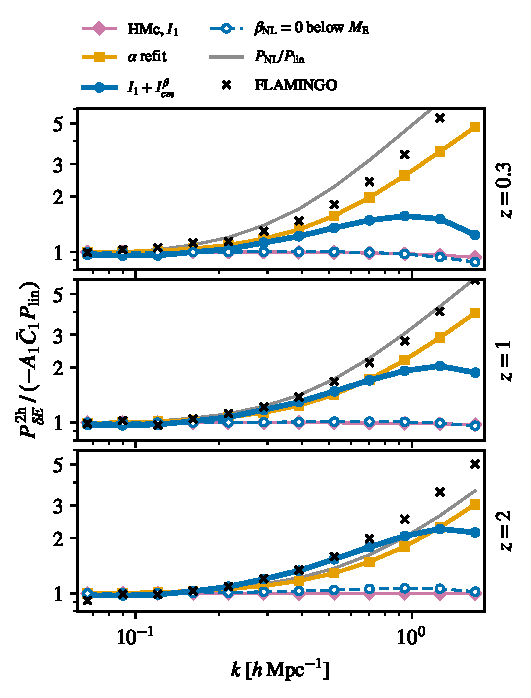
\includegraphics[width=3.5in]{plots/gi_kernel/gi_kernel.pdf}
  \caption{The GI 2-halo spectrum per unit $-A_1\Cb\Plin$. Pink diamonds:
  HMc ($I_1$); orange squares: the $\alpha$ refit at $\kmax = 0.70$; blue
  circles: $I_1 + \Ib{cm}$ with $\bNL$ held below the emulator's masses;
  dashed, open: $\bNL = 0$ below them; gray: $\PNL/\Plin$; crosses: FLAMINGO's
  $P_{\delta E}$ over $-A_1^{\rm NLA}\Cb\Plin$ with the NLA amplitude fitted at
  $\kmax = 0.22$ (all terms of the data, so it lies above the $A_1$ part
  alone). Error bars are smaller than the markers. The $z = 2$ curves use the
  $z = 1.48$ table.}
  \label{fig:kernel}
\end{figure}

The redshift trend of $\alpha$ follows. Written as an $\alpha$, $\Bigl.\Ib{cm}/(\PNL/\Plin - I_1)$ at
$k = 0.39$ rises from \AlphaBetaLowZ{} at $z = 0.2$ to \AlphaBetaZone{} at
$z = 1$, as the fitted $\alpha$ rises from 0.44 to 0.58; halos of fixed mass
are rarer at higher $z$, and their $\bNL$ is larger relative to the matter's
own nonlinearity.

\section{A check on FLAMINGO's clustering}
\label{sec:checks}

The held $\bNL$ matches FLAMINGO's measured galaxy-matter spectrum, and the
lower bracket does not (Fig.~\ref{fig:checks}). At $z = 1.5$ and 2, where
$P_{gm}$ was measured with the dark-matter particles, the halo model with
$\bNL$ is \PgmNlb{} of FLAMINGO at $k = 0.29$ to 0.94; without $\bNL$ it is
\PgmPlain{}, and with $\bNL = 0$ below $10^{12.6}\Msun$ \PgmLo{}. The same
holds for the matter spectrum against $\PNL$: \PmmNlbZone{} with $\bNL$ and
\PmmPlainZone{} without at $z = 1$, \PmmNlbZlow{} with $\bNL$ at $z = 0.3$.
The galaxy spectrum is overpredicted at $z = 1$ (\PggNlbZone{}, against
\PggPlainZone{} without $\bNL$); it depends on $\bNL$ for the lowest-mass
pairs twice and on the HOD's satellite term, which was fixed by $\nbar_g$
and $b_g$ only. These checks use no IA data.

\begin{figure}[tbp]
  \centering
  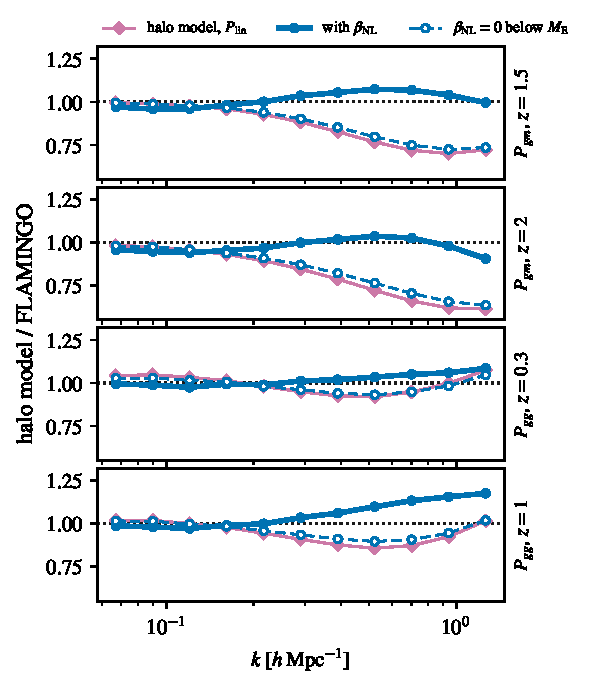
\includegraphics[width=3.5in]{plots/bias_checks/bias_checks.pdf}
  \caption{The halo model over FLAMINGO for the galaxy-matter spectrum
  ($z = 1.5$, 2) and the galaxy spectrum ($z = 0.3$, 1). Pink diamonds:
  2-halo on $\Plin$; blue circles: with $\bNL$; dashed, open: $\bNL = 0$
  below the emulator's lowest mass. Dotted: equality. The 1-halo terms come
  from the HMc HOD.}
  \label{fig:checks}
\end{figure}

\section{Fits without \texorpdfstring{$\alpha$}{alpha}}
\label{sec:fits}

Without $\alpha$ the model fits FLAMINGO only to $\kmax \approx 0.4$
(Fig.~\ref{fig:gof}). With $\bTA$ free the summed $\chi^2/\nu$ is \GofNlb{}
at $\kmax = 0.52$, 0.70 and 0.94; HMc gives \GofLin{} and the $\alpha$ refit
\GofAlpha{}. $\bNL$ improves on HMc for $\kmax \le 0.70$ and loses to it at
0.94, where its turnover costs more than HMc's flat deficit. With $\bTA = 0$
the result is \GofNlbTT{}, and in the NLA form ($A_2 = \bTA = 0$)
\GofNlbNLA{}, against \GofAlphaNLA{} for the NLA form with $\alpha$. With
$\bNL = 0$ below the emulator's masses ($\bTA = 0$) it is \GofNlbLo{}. The
shape-bias weight matters little: $w = 1$ changes the summed $\chi^2/\nu$ by
less than 2\%.

\begin{figure}[tbp]
  \centering
  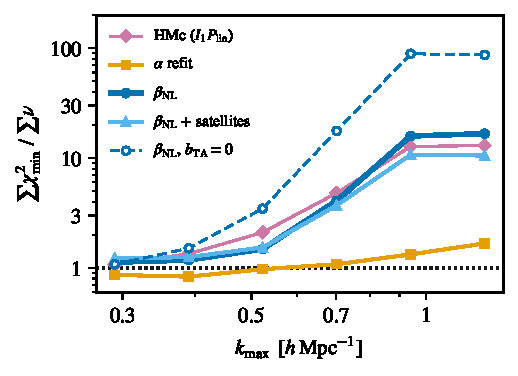
\includegraphics[width=3.5in]{plots/fit_gof/fit_gof.pdf}
  \caption{Summed $\chi^2_{\min}/\nu$ over the nine core snapshots against
  $\kmax$, all with $a_c \le 1$ and a free white term. Pink diamonds: HMc;
  orange squares: the $\alpha$ refit; blue circles: $\bNL$ with $\bTA$ free;
  sky-blue triangles: the same with the F21 satellites; dashed, open: $\bNL$
  with $\bTA = 0$. Dotted: $\chi^2/\nu = 1$, which is not a goodness-of-fit
  threshold here (the errors are underestimated at high $k$).}
  \label{fig:gof}
\end{figure}

\paragraph{Physical-sensibility checks} (Fig.~\ref{fig:params},
\texttt{nlbias\_numbers\_log.txt}).
\begin{itemize}[itemsep=1pt,topsep=2pt]
  \item \emph{Passed:} $A_1$ is \AoneRatioNlb{} times the low-$k$ NLA value
    for $\kmax \le 0.70$ at every snapshot (about 4 at $z = 1$). The low-$k$
    limit is NLA/TATT. In every best fit, $P_{EE}$ and $P_{BB}$ are positive
    at all measured $k$, and the GI and II 2-halo terms keep their sign below
    $k = 3\hMpc$.
  \item \emph{Failed, above the fit range:} at $k \ge 3\hMpc$ the GI 2-halo
    term changes sign in \NSignGI{} and the II 2-halo term in \NSignII{} of
    the 117 fits: exclusion removes the $A_1$ 2-halo term there and the
    one-loop $A_2$ and $\bTA$ terms take over.
  \item \emph{Failed, drift:} at $\kmax = 0.94$, $A_1$ falls to
    \AoneRatioNlbHigh{} of the NLA value and $\bTA$ rises from \bTANlbLow{}
    ($\kmax \le 0.52$) to \bTANlbHigh{}, against \bTAAlpha{} in the
    $\alpha$ refit at 0.94 with no trend in $\kmax$; $A_2$ grows more
    negative. $a_c$ sits at its bound of 1 in most fits: the model wants more
    1-halo power.
  \item \emph{Failed, satellites:} adding the F21 radial satellites gives
    \GofNlbSat{}; where nonzero, $a_{1h}$ is \AoneHSat{} and jumps between
    fit ranges, mostly above 0.3, where every satellite inside $r_{\rm vir}$
    has the capped alignment $\gamma_{\max} = 0.3$. The F21 term does not have
    the shape of the missing power.
\end{itemize}

\begin{figure}[tbp]
  \centering
  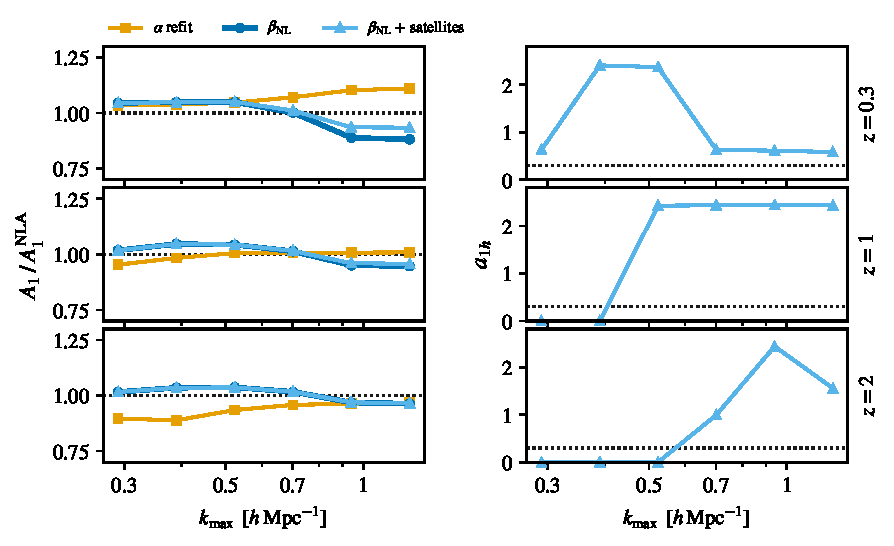
\includegraphics[width=6.4in]{plots/fit_params/fit_params.pdf}
  \caption{Left: $A_1$ over the NLA amplitude fitted at $\kmax = 0.22$,
  against $\kmax$, for the $\alpha$ refit (orange squares), $\bNL$ with
  $\bTA$ free (blue circles) and with satellites (sky-blue triangles).
  Right: the satellite amplitude $a_{1h}$ of the fit with satellites.
  Dotted: $A_1 = A_1^{\rm NLA}$ (left) and $a_{1h} = 0.3$, above which the
  satellite alignment is at its cap inside $r_{\rm vir}$ (right).}
  \label{fig:params}
\end{figure}

\section{Recommendation}
\label{sec:recommendation}

$\bNL$ is the physics behind about half of $\alpha$, the 2-halo half at
$k \lesssim 0.7$, and it explains why $\alpha$ rises with redshift. It does
not replace $\alpha$, because FLAMINGO's GI signal at $k \gtrsim 0.7$ is
1-halo power with the shape of $\PNL$, which neither the 2-halo term nor the
present 1-halo terms provide. The next steps, in order:
\begin{enumerate}[itemsep=1pt,topsep=2pt]
  \item Measure in FLAMINGO the central-shape cross with matter per host mass
    bin, $P_{\gamma_c m}(k|M)$, down to $10^{11.5}\Msun$. It tests the
    assumption $\beta^{Kh} = \bNL$, replaces the emulator's low-mass
    extrapolation, and splits the signal at $k \gtrsim 0.7$ into 2-halo and
    own-halo parts directly.
  \item Build the 1-halo GI term from that split: the central's alignment
    with the matter of its own halo beyond the triaxial quadrupole
    (substructure, the halo's outer shape), whose amplitude $a_c$ capped at 1
    cannot reach the data.
  \item Keep the $\alpha$ refit as the working model meanwhile; with $\bNL$
    in place, the remaining $\alpha$ would describe only the 1-halo part.
\end{enumerate}

\appendix

\section{Numerical checks}
\label{app:checks}

\begin{itemize}[itemsep=1pt,topsep=2pt]
  \item The $\alpha$ refit recomputed here (\texttt{alpha\_tatt}) gives the
    stored summed $\chi^2/\nu$ of \texttt{alpha\_cap\_nosat} to 0.01 at every
    $\kmax$.
  \item CAMB 2.0.5 here gives $\Plin$ 0.9\% above the stored v6 tables at
    $k > 0.05$; the fits use the stored $\Plin$ and $I_1$, and the $\bNL$
    integrals use the local CAMB (effect below 1\% on $\Ib{}$).
  \item $I_1$ and $b_g$ recomputed here agree with v6 to $10^{-15}$ and
    $10^{-3}$.
  \item Pair normalisation of $\bNL$: the large-scale cross-correlation
    coefficients of the emulator's mass bins lie between 0.93 and 1.03.
  \item For $z = 1.5$ and 2, assigning the $z = 1.48$ table to the same
    masses instead of the same peak heights changes the per-snapshot
    $\chi^2/\nu$ ($\bTA = 0$) from 1.96 to 1.96 ($z = 1.5$) and from 2.09 to
    2.14 ($z = 2$) at $\kmax = 0.52$, and from 8.30 to 8.24 and 5.80 to 4.99 at
    0.70.
  \item The $\alpha$ refit's GI 2-halo term changes sign below $k = 3$, and
    its $P_{EE}$ turns negative at $k \ge 3$, only in fits with
    $\kmax \le 0.16$, where $\alpha$ sits near its bound $-1$; none of the
    quoted $\alpha$ fits is affected.
\end{itemize}

\section{Where the code and results are}
\label{app:code}

All in \texttt{analysis/halo\_nlbias/} (the \texttt{README.md} gives run times).

\begin{center}\small
  \begin{tabular}{ll}
    \toprule
    result & script $\rightarrow$ output \\
    \midrule
    $\bNL(k, M_1, M_2)$ from Dark Emulator & \texttt{beta\_tables.py} $\rightarrow$ \texttt{beta\_tables.npz} \\
    halo-model integrals $I$, $\Ib{XY}$ & \texttt{halo\_nlbias.py} $\rightarrow$ \texttt{nlbias\_tables.npz} \\
    fits of every variant & \texttt{nlbias\_fit.py} $\rightarrow$ \texttt{nlbias\_fits.json} \\
    every quoted number, checks & \texttt{nlbias\_numbers.py} $\rightarrow$ \texttt{nlbias\_numbers.json} \\
    figures & \texttt{plots/make\_figure\_data.py} $\rightarrow$ \texttt{plots/*/data.json} \\
    \bottomrule
  \end{tabular}
\end{center}

\section{Open issues}
\label{app:open}

\begin{itemize}[itemsep=1pt,topsep=2pt]
  \item The assumption that halo shapes carry the nonlinear bias of halo
    positions ($\beta^{Kh} = \bNL$) is untested.
  \item $\bNL$ below $10^{12.6}\Msun$ is an extrapolation, and most centrals
    are there; $P_{gm}$ supports holding it, $P_{gg}$ at $z = 1$ suggests it
    is somewhat too high.
  \item The dip $\Ib{cm} \approx -0.03$ at $k = 0.1$ is not in $\PNL$; it comes
    from unequal-mass pairs of the emulator and was not traced further.
  \item The $z = 1.5$ and 2 tables extrapolate the emulator from $z = 1.48$.
  \item The fits use $P_{hE} = b(k)P_{\delta E}$; the halo-model galaxy-shape
    spectrum, Eq.~\eqref{eq:he}, was computed but not fitted.
  \item The Roman scale cuts and biases were not rerun with this model.
\end{itemize}

\end{document}
